\documentclass{article}
\usepackage[english, russian]{babel}
\usepackage{geometry}
\usepackage{abstract}
\usepackage{array}
\usepackage{graphicx}
\usepackage{enumitem}
\usepackage{cancel}
\usepackage{amsmath}
\usepackage{amssymb}
\usepackage{graphicx}
\usepackage{mathtools}
\usepackage{blindtext}
\usepackage[linktoc=none]{hyperref}
\usepackage{fancyhdr}

\newcommand{\mysection}[3]{\setcounter{section}{#1}\setcounter{subsection}{#2}\addtocounter{subsection}{-1}\subsection{#3}}

\title{\bf{Домашняя контрольная работа по математическому анализу}}
\author{Григорьев Данила Евгеньевич, 151 группа, "Программная инженерия" \and Преподаватель: Сахно Людмила Владимировна}
\date{22 февраля 2024 г.}

\geometry{
    a4paper,
    total={170mm,257mm},
    left=20mm,
    top=20mm,
}
\begin{document}
\pagestyle{fancy}
\maketitle

\begin{abstract}
    Вариант контрольной работы - 8. Выполнены задания: 1.10, 2.7, 3.9, 4.4, 5.7, 6.5
\end{abstract}

\tableofcontents
\newpage
\section*{Вариант 8}
\mysection{1}{10}{Вычислить производную функции}
\begin{enumerate}
    \item{\begin{math}
        y = 5 x \cos x \\
        y' = 5 \cos x + 5 x (- \sin x)
    \end{math}};
    
    \item{\begin{math}
        y = (\sqrt{2})^x + (\sqrt{5})^{x} \\
        y' = \dfrac 1 2 (\sqrt{2})^x \ln\sqrt{2} + \dfrac {-1} {2} (\sqrt{5})^{-x} \ln\sqrt{5}(-1)
    \end{math}};

    \item{\begin{math}
        y = \ln\ln\dfrac{x}{2} \\
        y' = \dfrac{1}{\ln\dfrac{x}{2}} \cdot \dfrac{1}{\dfrac{x}{2}} \cdot \dfrac{1}{2}
    \end{math}};

    \item{\begin{math}
        y = x - \ln\sqrt{1+e^{2x}}+e^{-x}\arcctg{e^x} \\
        y' = 1 - \dfrac{1}{\sqrt{1+e^{2x}}} \cdot \dfrac{1}{2\sqrt{1+e^{2x}}} * e^{2x} * 2 + e^{-x}(-x)\arcctg{e^x} + e^{-x} \cdot \dfrac{-1}{1+e^{2x}} \cdot e^x.
    \end{math}}
\end{enumerate}

\clearpage
\mysection{2}{7}{Вычислить производную функции, заданной неявно}
Дана функция $x^2-1+\cos{xy} = 0$. Вычислим производные $y'_x$ и $y''_{x^2}$.
\begin{enumerate}
    \item Решим уравнение производной первого порядка $y'_x$:
        \begin{equation*}
            (x^2-1+\cos{xy} = 0)'_x \Leftrightarrow 2x-\sin{xy}(y+xy') = 0.
        \end{equation*}
        \begin{equation*}
            y' = \dfrac{1}{x} \cdot \Bigg( \dfrac{2x}{\sin{xy}} - y \Bigg)
        \end{equation*}
    \item Решим уравнение производной второго порядка $y''_{x^2}$:
\begin{equation*}
(x^2-1+\cos{xy} = 0)''_x \Leftrightarrow
\big(2x-\sin{xy}(y+xy') = 0)'_x \Leftrightarrow
\end{equation*}
\begin{equation*}
\Leftrightarrow
2 - (\cos{xy}(y+xy')^2 + \sin{xy}(y'+y'+xy'' \cdot y')) = 0 \Leftrightarrow
2 - \cos{xy} \cdot (y+x)^2+\sin{xy} \cdot (2y'+xy'') = 0.
\end{equation*}
\begin{equation*}
    \sin{xy} \cdot (2y'+xy'') = \cos{xy} \cdot (y+x)^2 - 2
\end{equation*}
\begin{equation*}
    2y'+xy'' = \tg{xy} \cdot (y+x)^2 - \dfrac{2}{\sin{xy}}
\end{equation*}
\begin{equation*}
    y'' = \dfrac{1}{x} \cdot \Bigg( \tg{xy} \cdot (y+x)^2 - \dfrac{2}{\sin{xy}} -2y' \Bigg)
\end{equation*}
\end{enumerate}

\clearpage
\mysection{3}{9}{Найти уравнение касательной и нормали к кривой в точке M}
Дано:
\begin{equation*}
f = f(x) = x^2\arcsin{\frac x 2}, \\
x=x_M=1
\end{equation*}
Решение:
\begin{equation*}
    y = f(x_0) + f'(x_0)(x-x_0).
\end{equation*}
\begin{enumerate}
    \item $f' = f'(x) = \Big(x^2\arcsin{\dfrac x 2}\Big)' = 2x\arcsin{\dfrac x 2} + \dfrac{x^2}{\sqrt{4-x^2}}$;
    \item $x_0 = 1 \Rightarrow y_0 = f(x_0) =1^2\arcsin{\frac 1 2} = \dfrac{\pi}{6}$;
    \item $f'(x_0) = f'(1) = 2 \cdot 1\arcsin{\dfrac{1}{2}} + \dfrac{1^2}{\sqrt{4-1^2}} = 
    \dfrac{\pi}{3} + \dfrac{\sqrt{3}}{3} = \dfrac{\pi + \sqrt{3}}{3}$
\end{enumerate}
Уравнение касательной к графику функции $f=f(x)$ в точке $M$:
\begin{equation*}
    y = \dfrac \pi 6 + (\dfrac{\pi + \sqrt{3}}{3})(x-1).
\end{equation*}
Общее уравнение нормали к графику функции $f=f(x)$ в точке $x=x_0$:
\begin{equation*}
    x-x_0+f'(x_0)(y-f(x_0))=0 \Leftrightarrow y = f(x_0) - \dfrac{x-x_0}{f'(x_0)}
\end{equation*}
\begin{equation*}
    y=\dfrac{\pi}{6} - \dfrac{x-1}{\dfrac{\pi + \sqrt{3}}{3}} = \dfrac{\pi}{6} - \dfrac{3x-3}{\pi + \sqrt{3}}.
\end{equation*}

\clearpage
\mysection{4}{4}{Представить формулой Маклорена с $\overline{o}(x^n)$ функцию $f(x)$}
Дано:
\begin{equation}
f(x)=\ln{\dfrac{2-3x}{3+2x}}
\end{equation}
Вспомним следующие формулы:
\begin{description}
    \item[Формула Тейлора.] $f(x) = \displaystyle\sum_{k=0}^{n}{\dfrac{f^{(k)}(x_0)}{k!}(x-x_0)^k} + \overline{o}((x-x_0)^n), x \to x_0$
    \item[Формула Маклорена.] $f(x) = \displaystyle\sum_{k=0}^{n}{\dfrac{f^(k)(0)}{k!} \cdot x^k} + \overline{o}(x^n), x \to 0$
    \item[Логарифмическая функция.] \, \\
        \begin{equation}
            \ln(1+x) = \displaystyle\sum_{k=1}^n \dfrac{(-1)^{k-1}x^k}{k} + \overline{o}(x^n) \\
        \end{equation}
        \begin{equation}
            \ln(1-x) = -\displaystyle\sum_{k=1}^n \dfrac{x^k}{k} + \overline{o}(x^n)
        \end{equation}
\end{description}
Упростим заданную функцию (1):
\begin{equation*}
    \ln{\dfrac{2-3x}{3+2x}} = \ln{\dfrac{2\Bigg(1-\dfrac{3x}{2}\Bigg)}{3\Bigg(1+\dfrac{2x}{3}\Bigg)}} = \ln\dfrac{2}{3} + \ln(1-\dfrac{3x}{2}) - \ln(1+\dfrac{2x}{3})
\end{equation*}
И представим её формулой Маклорена с помощью формул (2) и (3): \\
\begin{equation*}
    f(x) = \ln{\dfrac{2}{3}} - \displaystyle\sum_{k=1}^n \dfrac{(3x)^k}{2^k k} + \displaystyle\sum_{k=1}^n \dfrac{(-1)^{k-1}(2x)^k}{3^k k} + \overline{o}(x^n) =
    \ln{\dfrac{2}{3}} + \displaystyle\sum_{k=1}^n \dfrac{(-1)^{k-1}(4x)^k - (9x)^k}{6^k k} + \overline{o}(x^n)
\end{equation*}

\clearpage
\mysection{5}{7}{Вычислить предел}
Вычислим предел, используя правило Лопиталя:
\begin{multline*}
\lim\limits_{x \to 0}\Bigg(\dfrac{1}{x^2}-\ctg^2 x\Bigg) = \lim\limits_{x \to 0}\Bigg(\dfrac 1 x^2 - \dfrac{\cos^2 x}{\sin^2 x}\Bigg) = \lim\limits_{x \to 0}\Bigg(\dfrac{\sin^2 x - \cos^2 x \cdot x^2}{x^2\sin^2 x}\Bigg) = \Bigg[\dfrac 0 0\Bigg] =\\
= \lim\limits_{x \to 0}\dfrac{2\sin x \cos x - (2\cos x(-\sin x)x^2 + \cos^2 x \cdot 2x)}{2x\sin^2 x + x^2 \cdot 2 \sin x \cos x}
= \lim\limits_{x \to 0}\dfrac{2(\sin x \cos x - x \cos x(-x\sin x + \cos x))}{2x\sin x(\sin x + x \cos x)} =\\
= \lim\limits_{x \to 0}\dfrac{\overset{\overset 1 \uparrow}{\overbrace{\cos x}}(\sin x - x(\cos x - x\sin x))}{x\sin x(\sin x + x \cos x)} = \lim\limits_{x \to 0}\dfrac{\sin x + x^2\sin x - x\cos x}{x(\sin x(\sin x + x \cos x))} = \Bigg[\dfrac 0 0\Bigg] =\\
= \lim\limits_{x \to 0}\dfrac{\cancel{\cos x} + 2x\sin x + x^2 \cos x \cancel{- \cos x} + x \sin x}{\sin x(\sin x + x \cos x) + x(\cos x(\sin x + x \cos x) + \sin x(\cos x + \cos x - x\sin x))} = \\
= \lim\limits_{x \to 0}\dfrac{3x\sin x + x^2 \cos x}{\sin^2 x + x \sin x \cos x + x \sin x \cos x + x^2 \cos^2 x + x \sin x \cos x - x \sin^2 x} =\\
= \lim\limits_{x \to 0}\dfrac{3x^2 + x^2\cos x}
{x^2 \underset{\underset 1 \downarrow}{\underbrace{\dfrac{\sin^2 x}{x^2}}}
+ x^2 \underset{\underset 1 \downarrow}{\underbrace{\dfrac{\sin x}{x}}} \cos x
+ x^2 \underset{\underset 1 \downarrow}{\underbrace{\dfrac{\sin x}{x}}} \cos x
+ x^2 \cos x + x^2 \underset{\underset 1 \downarrow}{\underbrace{\dfrac{\sin x}{x}}} \cos x
- x^4 \underset{\underset 1 \downarrow}{\underbrace{\dfrac{\sin^2 x}{x^2}}}} =\\
= \lim\limits_{x \to 0}\dfrac{3x^2 + x^2\cos x}{x^2 + x^2\cos x + 3x^2\cos x - x^4} = \lim\limits_{x \to 0}\dfrac{3+\cos x}{1 + \cos x + 3 \cos x - x^2} = \dfrac 4 6 = \dfrac 2 3.
\end{multline*}

\clearpage
\mysection{6}{5}{Исследовать функцию и начертить график}
Дана функция $f(x) = x - \sqrt{x^2 - 2x}$. Исследуем функцию в соответствии со схемой построения её графика:
\begin{description}
\item[Область определения.] $D(f) = (-\infty;0]\cup[2;+\infty)$;
\item[Чётность.] $f(-x) = -x - \sqrt{x^2+2x}$, $-f(x) = -x + \sqrt{x^2 - 2x}$ $\Rightarrow f(-x) \not= -f(x) \land f(-x) \not= f(x) \Rightarrow f~\textrm{-- функция общего типа;}$
\item[Периодичность.] $\forall t \in \mathbb{R}~\exists x_0 \in D(f): f(x_0+t)\ne f(x_0)\Rightarrow f~\textrm{не периодическая;}$
\item[Промежутки знакопостоянства.] Найдём промежутки знакопостоянства, решив неравенства.
\begin{enumerate}
\item Рассмотрим случай, когда $f(x) < 0$:
\begin{equation*}
    x - \sqrt{x^2-2x} < 0
\end{equation*}
\begin{equation*}
    x < \sqrt{x^2-2x}
\end{equation*}
\begin{equation*} \begin{cases*} x < 0 \\ x^2 - 2x \geq 0 \end{cases*}\begin{cases*} x < 0 \end{cases*} \end{equation*}
\item Рассмотрим случай, когда $f(x) > 0$:
\begin{equation*}
    x - \sqrt{x^2-2x} > 0
\end{equation*}
\begin{equation*}
    x > \sqrt{x^2-2x}
\end{equation*}
\begin{equation*} \begin{cases*} x > 0 \\ x^2 - 2x \geq 0 \\ x^2 - 2x < x^2 \end{cases*}\begin{cases*} x > 0 \\ x(x-2) \geq 0 \end{cases*} \begin{cases*} x \geq 2 \end{cases*} \end{equation*}
\end{enumerate}
$\forall x \in (-\infty; 0)~f(x) < 0;~\forall x \in [2; +\infty)~f(x) > 0;$
\item[Горизонтальные асимптоты.]
    $y = 1$ является горизонтальной асимптотой, так как
    \begin{equation*}
        \lim\limits_{x \to +\infty}{f(x)} = \lim\limits_{x \to +\infty}(x - \sqrt{x^2-2x}) = \lim\limits_{x \to +\infty}\dfrac{x^2-x^2+2x}{x+\sqrt{x^2-2x}} = \dfrac{2}{1+\sqrt{1}} = \dfrac 2 2 = 1
    \end{equation*}

\item[Наклонные асимптоты.] Составим уравнение наклонной асимптоты вида $y = kx + b$, где $k, b \in \mathbb{R}:$
    \begin{enumerate}[start=3]
        \item $k = \lim\limits_{x \to -\infty}{\dfrac {f(x)} {x}} = \lim\limits_{x \to -\infty}{\dfrac{x-\sqrt{x^2-2x}}{x}} = \lim\limits_{x \to \infty}{\dfrac{-x-\sqrt{x^2+2x}} {-x}} = \lim\limits_{x \to \infty}\Bigg(1 + \sqrt{1 + \dfrac 2 x}\Bigg) = 2;$
        \item $b = \lim\limits_{x \to -\infty}{(f(x) - kx)} = \lim\limits_{x \to -\infty}{x - \sqrt{x^2-2x} - 2x} = \lim\limits_{x \to \infty}{-x - \sqrt{x^2+2x} + 2x} = \lim\limits_{x \to \infty}{x - \sqrt{x^2+2x}} = \lim\limits_{x \to \infty}\dfrac{x^2 - x^2 - 2x}{x + \sqrt{x^2+2x}} = \lim\limits_{x \to \infty}\dfrac{-2}{1 + \sqrt{1+\dfrac 2 x}} = \dfrac{-2}{2} = -1;$
    \end{enumerate}
    Значит, существует наклонная асимптота  $y = 2x - 1$ при $x \to -\infty.$

\item[Исследование на монотонность и локальные экстремумы.] Найдём $f'(x)$:
    \begin{equation*}
        f'(x) = 1 - \dfrac{2x - 2}{2\sqrt{x^2 - 2x}} = 1 - \dfrac{x - 1}{\sqrt{x^2 - 2x}};
    \end{equation*}
    Найдём стационарные точки, решив уравнение:
    \begin{equation*}
        f'(x) = 0 \Leftrightarrow 1 - \dfrac{x - 1}{\sqrt{x^2 - 2x}} = 0;
    \end{equation*}
    \begin{equation*}
        x - 1 = \sqrt{x^2 - 2x}, x \in \mathbb{R} \backslash (0,2)
    \end{equation*}
    \begin{equation*}
        x^2 - 2 = x^2 - 2x
    \end{equation*}
    \begin{equation*}
        2x = 2
    \end{equation*}
    \begin{equation*}
        x = 1 \notin \textrm{ОДЗ} \Rightarrow \textrm{нет корней} \Rightarrow \textrm{нет точек экстремума}
    \end{equation*}
    В связи с отсутствием точек экстремума, вычислив значение функции $f'(x)$ для произвольного элемента из полуинтервала $(-\infty;0]$, установим, что
    \begin{equation}
        \forall x \in (-\infty;0] f'(x) > 0 \Leftrightarrow f(x) \textrm{ возрастает на полуинтервале} (-\infty;0];
    \end{equation}
    Аналогично для полуинтервала $[2;+\infty)$:
    \begin{equation}
        \forall x \in [2;\infty) ~ f'(x) < 0 \Leftrightarrow f(x) ~ \textrm{ убывает на полуинтервале} ~ [2;\infty);
    \end{equation}

\item[Исследование на выпуклость и перегибы.] Найдём $f''(x)$:
    \begin{equation*}
        f''(x) = \dfrac{-1}{\sqrt{(x^2-2x)^3}};
    \end{equation*}
    Поскольку уравнение $f''(x) = 0$ не имеет корней, у исследуемой функции нет точек перегиба. По аналогии с исследованием на монотонность функции, исследуем её на выпуклость:
    \begin{equation}
        \forall x \in (-\infty;0] ~ f''(x) > 0 \Leftrightarrow f(x) ~ \textrm{ -- выпуклая вверх на полуинтервале} ~ (-\infty;0];
    \end{equation}
    \begin{equation}
        \forall x \in [2;\infty) ~ f''(x) > 0 \Leftrightarrow f(x) ~ \textrm{ -- выпуклая вверх на полуинтервале} ~ [2;\infty);
    \end{equation}
    Таким образом, $f(x)$ является выпуклой на всей своей области определения.
\item[График функции.] На основании полученных ранее данных, построим график функции $y = f(x)$\\
\begin{figure}[h]
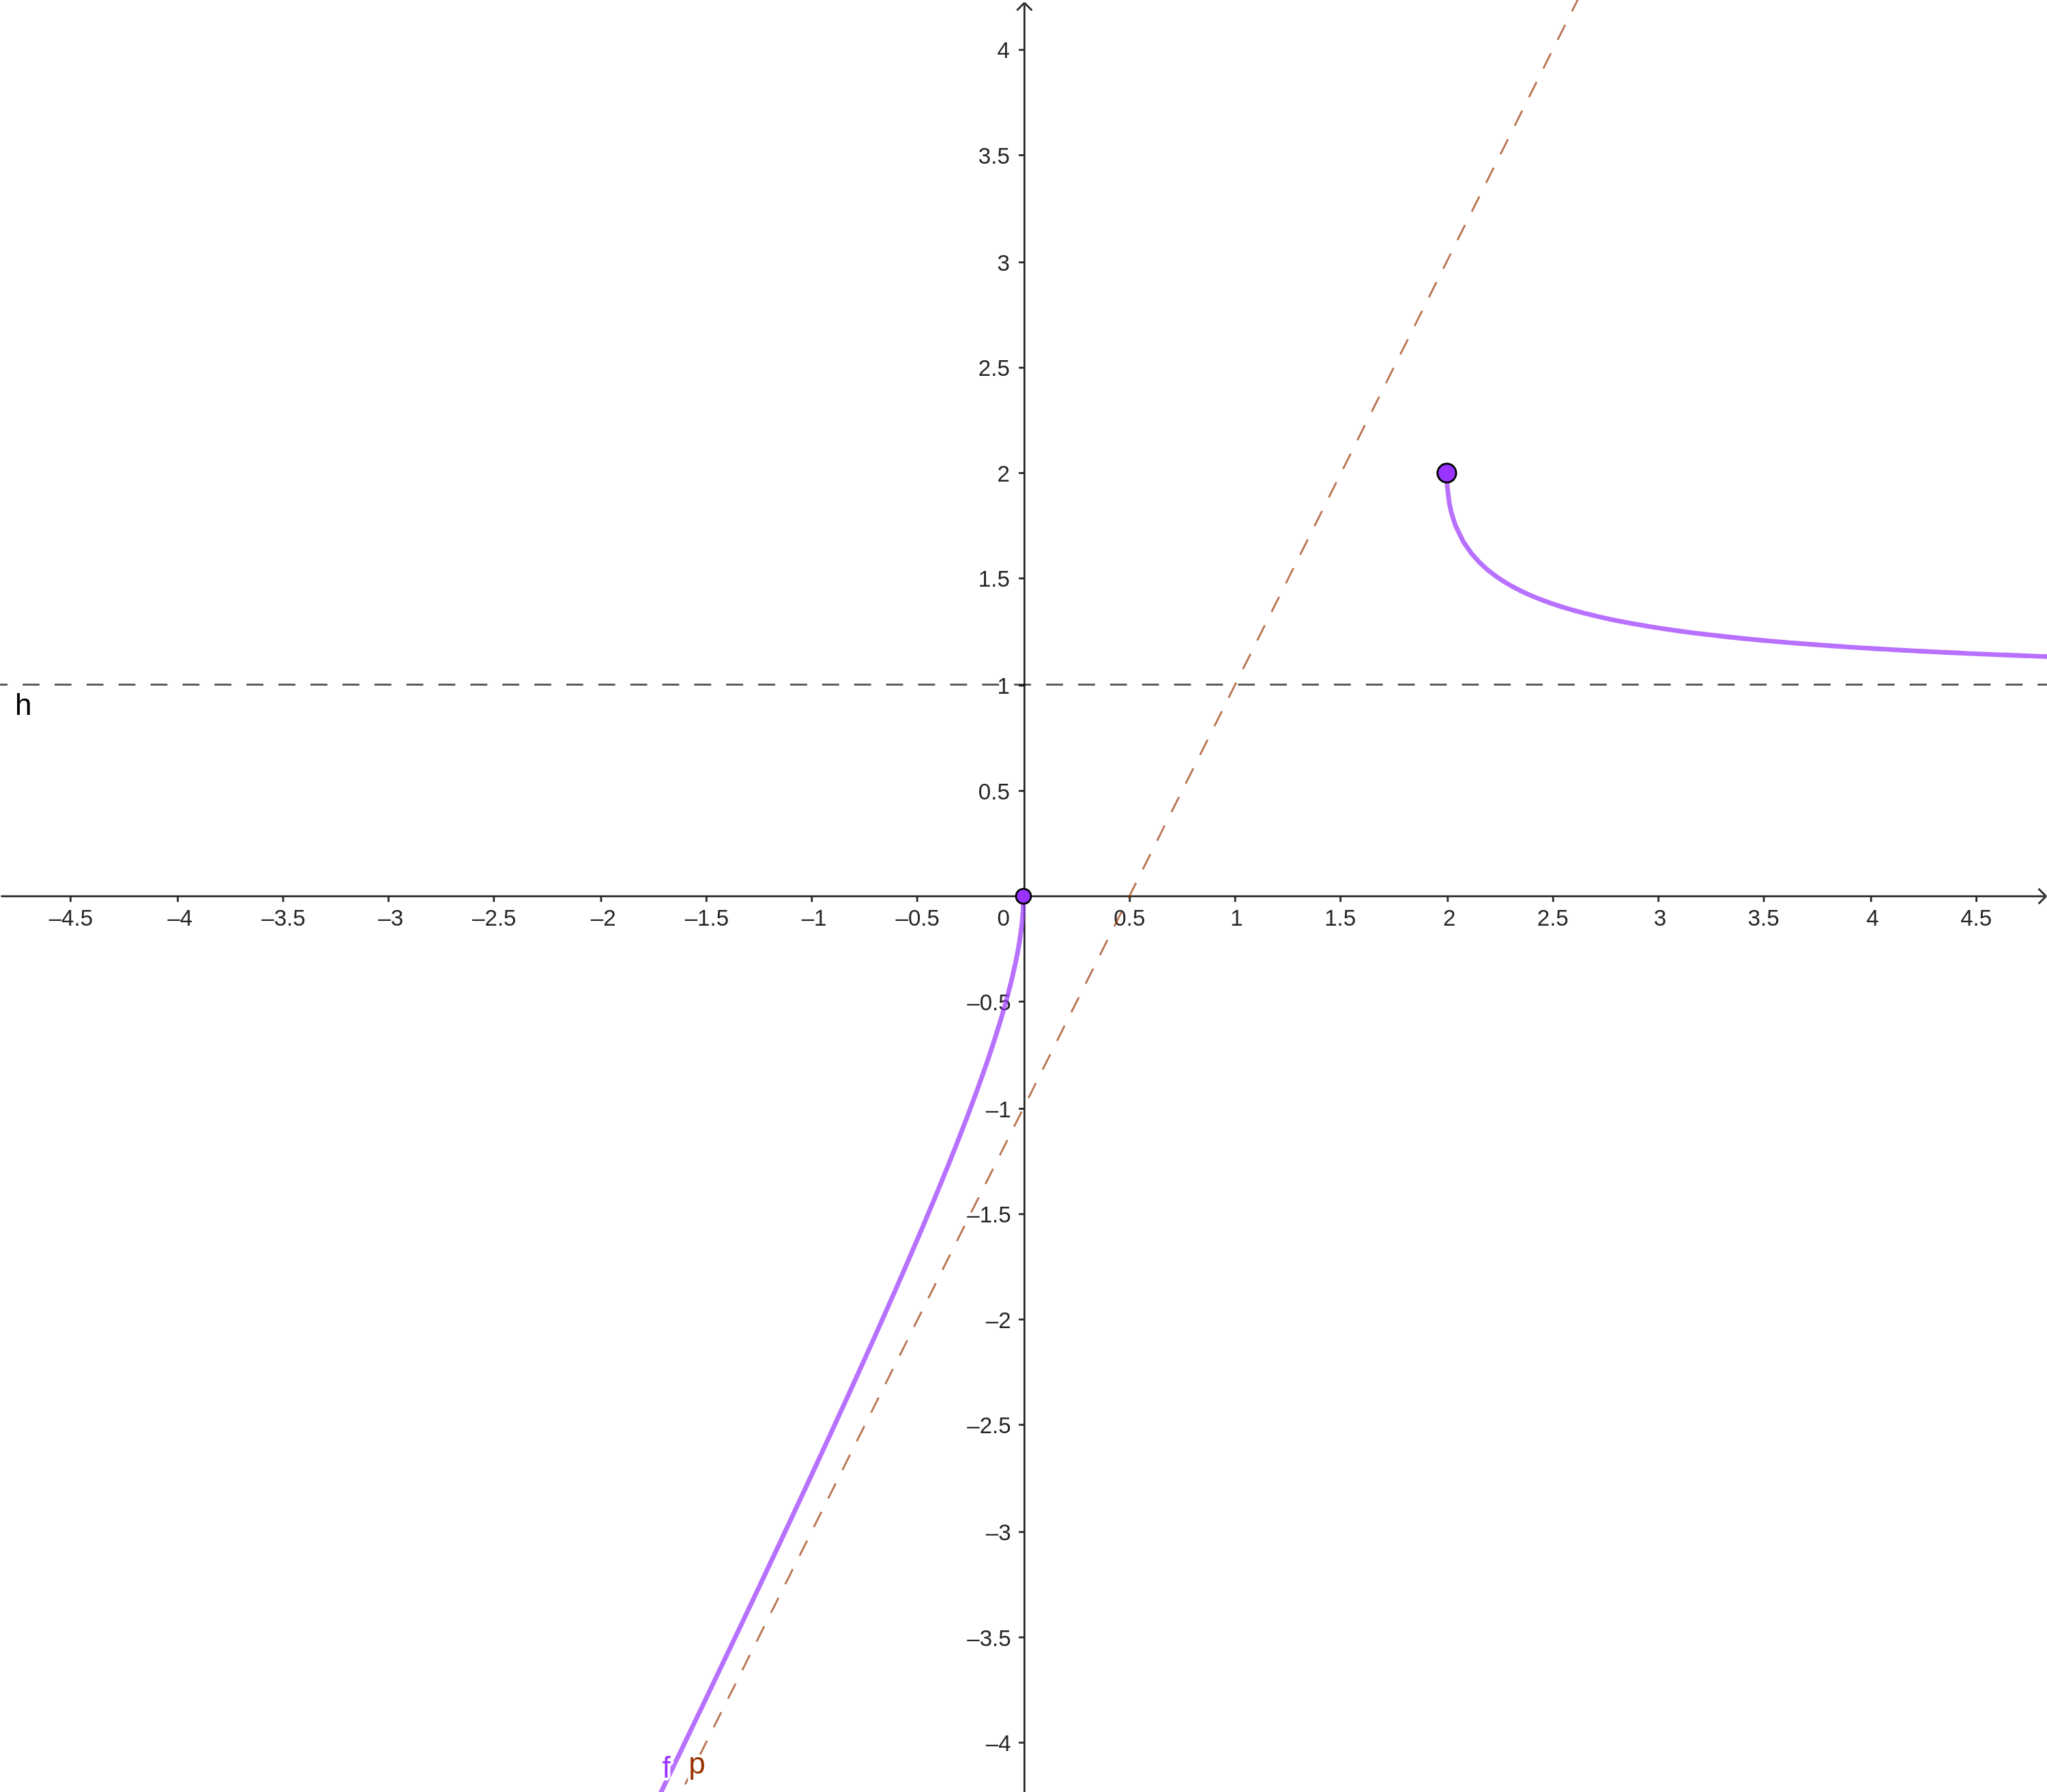
\includegraphics[width=\textwidth]{кр_6.png}
\end{figure}
\end{description}


\newpage
\end{document}